\subsection{Dynamic Time Warping}
\label{dtw}

The question of how to take the difference between the demand curve and
the production curve is an important one. The na\"ive option is to simply
take the $L_1$ norm of the difference between these two time series, as
seen in Equation \ref{delta-l1}.  However, since the $g(t, \Theta)$ computed
from a simulation is expensive, any operation that can meaningfully
exacerbate the difference between time series helps drive down the number
of optimization iterations.

Dynamic time warping is just such a mechanism. It computes
a distance between any two time series which compounds the separation
between the two. Additionally, the time series are not required to be of the
same length, though for optimization purposes there is no reason for them
not to be. DTW gives a measure of the amount that one time series would need to
be warped to become the other time series. It is, therefore, a holistic
measure that operates over all times. Dynamic time warping
is more fully covered in \cite{muller}.  However, an
optimization-relevant introduction is given here.

For the time series $f$ and $g$, there are three parts to dynamic time
warping. The first is the distance $d$, which will be minimized. The second
is a cost matrix $C$ that helps compute $d$ by indicating how far a point
on $f$ is from another point on $g$. Thirdly, the warp path $u$ is the
minimal cost curve through the $C$ matrix from the fist point in time to
the last. The DTW distance can thus be interpreted as the
total cost of traveling the warp path.

The first step in computing a dynamic time warp distance is to
assemble the cost matrix. Say that the demand time series $f$ has
length $A$ indexed by $a$, and the production time series $g$ has
length $B$ indexed by $b$. For the optimization problem here, $A$ and $B$
are in practice both equal to $T$.  However, it is useful to have $a$ and
$b$ index the two time series separately. Now denote an $A\times B$ matrix
$\Delta L$ as the $L_1$ norm of the difference between $f$ and $g$:
\begin{equation}
\label{delta-l1}
\Delta L_{a,b} = \left|f(a) - g(b, \Theta)\right|_1
\end{equation}
Since $\Delta L$ uses the $L_1$ norm, $f$ and $g$ may return vector
data. This enables multi-objective optimization. However it is recommended
that the components of the $f$ and $g$ are weighted, normalized, or otherwise
directly comparable.

The cost matrix $C$ may now be defined as the $A\times B$ sized matrix
which follows the recursion relations seen in Equation \ref{cost-matrix}.
\begin{equation}
\label{cost-matrix}
\begin{split}
C_{1,1} & = \Delta L_{1,1}\\
C_{1,b+1} & = \Delta L_{1,b} + C_{1,b}\\
C_{a+1,1} & = \Delta L_{a,1} + C_{a,1}\\
C_{a+1,b+1} & = \Delta L_{a,b} + \min\left[C_{a,b}, C_{a+1,b}, C_{a,b+1}\right]
\end{split}
\end{equation}
The boundary conditions above are the same as setting an infinite cost to
any $a \le 0$ or $b \le 0$. The cost matrix $C$ has the same units as the
demand curve. However, the scale of $C$ is
larger than the demand,
except for in the fiducial case. This is because the cost matrix compounds the
minimum value of previous entries.

Knowing a cost matrix, the warp path can be computed by traversing the
matrix backwards from the $(A, B)$ corner to the $(1, 1)$ corner.
If the length of the warp is $I$ indexed by $i$, the warp path itself
can be thought of as a sequence of coordinate points $u_i$. For a given
point $u_i$ in the warp path, the previous point $u_{i-1}$ may be found by
picking the minimum cost point among the locations one column over $(a,b-1)$,
one row over $(a-1,b)$, and one previous diagonal element to $(a-1,b-1)$.
Equation \ref{warp-path} expresses this mathematically.
\begin{equation}
\label{warp-path}
u_{i-1} = \argmin\left[C_{a-1,b-1}, C_{a-1,b}, C_{a,b-1}\right]
\end{equation}
The maximum possible length of $u$ is thus $\max(I) = A + B$.
The minimum possible length, though, is $\min(I) = \sqrt{A^2 + B^2}$.

The dynamic time warping distance distance $d$ can now be stated as the
cost of the final entry of the warp path normalized by the maximum possible
length of the warp path.
\begin{equation}
\label{d-calc-ab}
d(f, g) = \frac{C_{A,B}}{A + B}
\end{equation}
However, because the demand curve and the production curve
are often defined on the same time grid, $d$ can be further
reduced to the following:
\begin{equation}
\label{d-calc}
d(f, g) = \frac{C_{T,T}}{2T}
\end{equation}
Therefore, $d$ has the same units as the demand curve, production curve,
and cost matrix.

As an example, take a 1\% growth that starts with 90 GWe in the year
2016 as the demand curve. Then consider a production curve that
under-produces the demand by 5\% for 25 years before switching to
over-producing this curve by 5\% for the next 25 years.
Figure \ref{cost-demand-to-production} shows the dynamic time warping
cost matrix between these two time series as a heat map.

\begin{figure}[htb]
\centering
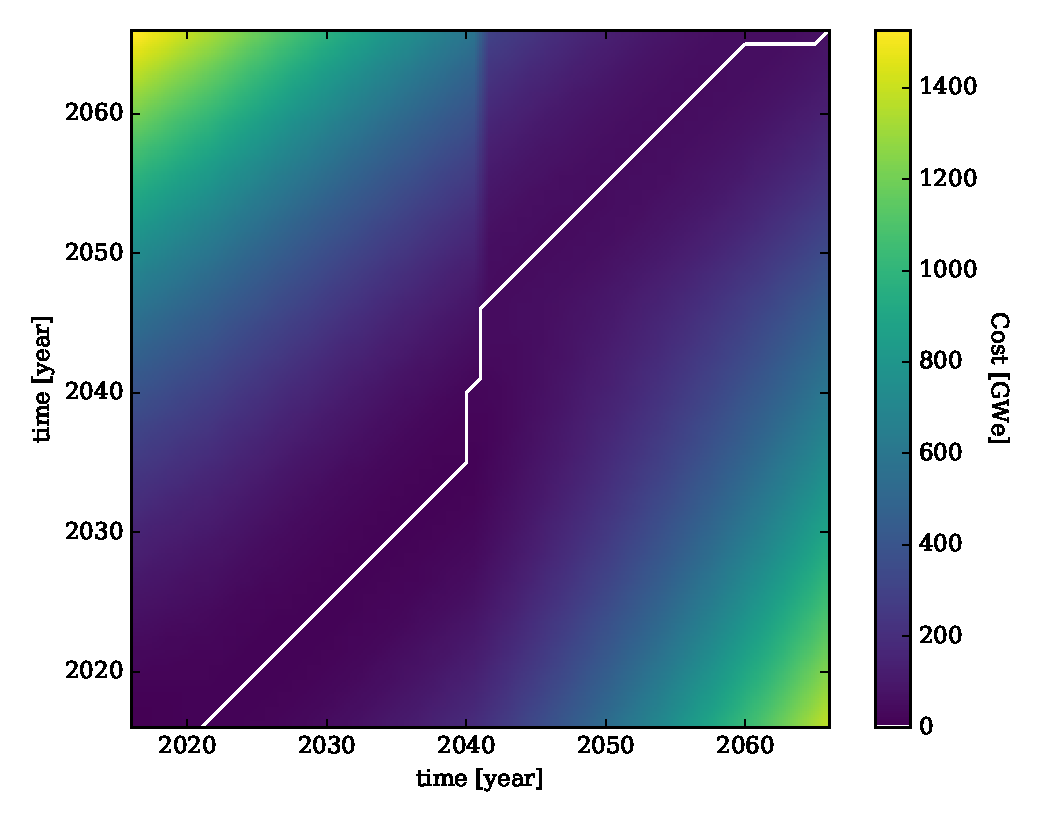
\includegraphics[width=0.9\textwidth]{cost-demand-to-production.eps}
\caption{Heat map of the cost matrix between a 1\% growth demand curve and
a production curve the under produces by 5\% for the first 25 years and then
over produces for the second 25 years.
The warp path $u$ is superimposed as the white curve on top of the
cost matrix.}
\label{cost-demand-to-production}
\end{figure}

Additionally, the warp path between the example demand and production
curves is presented as the white curve on top of the heat map in
Figure \ref{cost-demand-to-production}.
Recognize that $u$ is monotonic along both time axes. Furthermore, the precise
path of $u$ minimizes the cost matrix at every step. Regions of increased
cost in the cost matrix can be seen to repel the warp path. The
distance $d$ between the demand and production curves here happens
to be 0.756 GWe.

Dynamic time warping distance can therefore be used as an objective function
to minimize for any demand and production curves. However, using full
simulations to find $g(t, \Theta)$ remains expensive, even though DTW itself
is computationally cheap. Therefore, a mechanism to reduce the overhead
from production curve evaluation is needed.
